\documentclass[12pt,a4paper]{article}

% include standard packages:
\usepackage{graphicx, epstopdf} % eps... for e.g. MATLAB-Grafiken im .eps-format
\graphicspath{{./img/}} % default folder for images

\usepackage[automake, toc]{glossaries}
\usepackage{acronym}
\usepackage{xcolor}
\usepackage[hyphens]{url} % fix too long urls in bibliography
\usepackage{hyperref} % [colorlinks,linkcolor=black,citecolor=black,urlcolor=black] % customize references
% uncomment the next lines to avoid red boarder around hyperlinks
% simple:
%\hypersetup{
%    colorlinks,
%    citecolor=black,
%    filecolor=black,
%    linkcolor=black,
%    urlcolor=black
%}
% advanced:
%\hypersetup{
%    pdftitle    = \mytitle,
%    pdfsubject  = \worktype,
%    pdfauthor   = \myname,
%    pdfcreator  = {pdflatex},
%    bookmarksnumbered = true,
%    colorlinks = true,
%    linkcolor = black,
%    citecolor = blue,
%    urlcolor = blue
%}

\usepackage{amsmath, amsfonts, amssymb, amsthm} % enhanced math writing
\usepackage{tikz-timing} % Timing, Square-Symbols
\usepackage[clock, weather, misc, alpine, geometry, electronic]{ifsym} % \showclock; \Sun; \Letter; \Hut; \FallingEdge
\usepackage{wasysym,gensymb,trfsigns} % Hantelsymb., gensymb for celsius ohm, usw.
\usepackage[tmargin=1in,bmargin=1in,lmargin=1.25in,rmargin=1.25in]{geometry} % MSWord-A4-Format
\setlength{\parindent}{0em} % keine Einrueckungen, sonst \noindent

%\usepackage{listings, lstautogobble} % adding code listing support
\usepackage[final]{listings}
\usepackage{accsupp}
\newcommand{\noncopynumber}[1]{%
    \BeginAccSupp{method=escape,ActualText={}}%
    #1%
    \EndAccSupp{}%
}
\lstset{
    captionpos=b, numberbychapter=false,caption=\lstname,frame=single, 
    numbers=left, stepnumber=1, numbersep=5pt, xleftmargin=10pt, 
    framexleftmargin=15pt, numberstyle=\tiny\noncopynumber, tabsize=3, columns=fixed, 
    basicstyle={\fontfamily{pcr}\selectfont\footnotesize}, keywordstyle=\bfseries, 
    commentstyle={\color[gray]{0.33}\itshape}, stringstyle=\color[gray]{0.25}, 
    breaklines, breakatwhitespace, breakautoindent
}
\lstloadlanguages{[ANSI]C, C++, [gnu]make, gnuplot, Matlab, VHDL}
\lstset{language=[ANSI]C}
\newcommand*\listingspath[1]{\lstset{inputpath=#1}}
\listingspath{./codes/} % default folder for codes

\usepackage{float} % improved inteferce of floating objects (e.g. \floatplacement{figure}{H})
\usepackage{sectsty} % apply different fonts for a section
\usepackage{eso-pic} % backround image e.g.
%\usepackage{ulem} % \uuline = Doppelt unterstreichen, do not use with bibliography
\usepackage{tikz} % drawing things
\usepackage{pgfplots} % plots, graphs, etc.

% customize Header and Footer
\usepackage{fancyhdr, lastpage}
\pagestyle{fancy}
\fancyhf{}
\lhead{Standard Template}
\rhead{Name}
\lfoot{\today}
\rfoot{Seite \thepage \space von \pageref{LastPage}}
\renewcommand{\headrulewidth}{0.4pt}
\renewcommand{\footrulewidth}{0.4pt}

% Umlaute-Encoding und Standardschrift einstellen:
\usepackage[ngerman]{babel} % ngerman for Januar in today
\usepackage[utf8]{inputenc}
\usepackage[T1]{fontenc}
\usepackage{lmodern} % avoid bitmap letters
% use standard font:
%\renewcommand\rmdefault{lmr}
%\renewcommand\sfdefault{lmss}
%\renewcommand\ttdefault{lmtt}

% Citation
\usepackage[autostyle=false, style=english]{csquotes}
\MakeOuterQuote{"}
%\usepackage[style=british]{csquotes}
%\usepackage[backend=bibtex, autolang=hyphen, style=authoryear]{biblatex}
%\addbibresource{bibliography.bib}
\usepackage[backend=biber, style=numeric]{biblatex}
\addbibresource{Literatur.bib}

% uncomment the following 2 lines to use Arial
%\usepackage{helvet}
%\renewcommand{\familydefault}{\sfdefault}
\providecommand\listacroname{}

% Rename listings
%\renewcommand{\contentsname}{Inhaltsverzeichnis}
\renewcommand{\lstlistlistingname}{Quellcodeverzeichnis} % Codelistings
%\renewcommand{\listfigurename}{Abbildungsverzeichnis}
%\renewcommand{\listtablename}{Tabellenverzeichnis}
\renewcommand\listacroname{Abkürzungsverzeichnis}

% Add listoffigures and codelistings in tableofcontents
\usepackage[nottoc]{tocbibind} %,numbib
\renewcommand{\lstlistoflistings}{\begingroup
	\tocfile{\lstlistlistingname}{lol}
\endgroup}

% Title page configuration
\title{Template}
\author{Jonas Berger}
\date{Published: \today \\ Updated: \today}

\renewcommand{\glossarysection}[2][]{}
\makeglossaries

\begin{document}
\maketitle
\thispagestyle{empty}
\pagebreak

\renewcommand{\abstractname}{Abstract} % if german-babel used change Abstractname here
\begin{abstract} % make Abstract
	\noindent
	Einleitung des Dokuments
\end{abstract}

\tableofcontents
\pagebreak

\section{Einleitung}

\begin{itemize}
	\item Kurze Einleitung zur Thema des Experimentes,
	\item Ziele des Experimentes.
	\item Beispiel Griechischer Buchstabe: $\vartheta$
\end{itemize}

\section{Theoretischer Hintergrund}
Hier müssen Sie ausfürlich darüber schreiben, alle 
Themen und Konzepte die Sie brauchen, um das 
Experiment verstehen und durchführen zu können.

\section{Experiment}
\label{sec:Experiment}

	\subsection{Beschreibung des Experimentes}
	Hier müssen Sie Ihr Experiment so detailliert beschreiben, 
	dass die Person, die Ihr Protokoll liest, und nicht bei Ihnen 
	das Experiment durchgeführt hat, genau das selbe 
	machen kann wie Sie, und die selbe Ergebnisse bekommen 
	kann, die Sie hier berichten.

	\subsection{Berechnungen}
	Bitte Ihre Berechnungen nie händisch hinzufügen!
	
	\begin{equation}\label{eq:1}
		x=-\frac{p}{2}\pm\sqrt{\left(\frac{p}{2}\right)^2-q}
	\end{equation}

	Hier wird auf die Formel  \ref{eq:1} verwiesen. %eqref{} ... (1)

	\subsection{Simulationen}
	Alles was Sie im Labor gemessen haben, müssen Sie 
	simulieren. Aber bitte nicht nur Abbildungen: beschreiben 
	Sie auch, was Sie simuliert haben.
		
	\pagebreak

	\subsection{Messungen / Ergebnisse}
	Fügen Sie Ihre Ergebnisse hier. Aber bitte nicht nur Abbildungen: Sie müssen auch beschreiben, wie Sie diese Ergebnisse 
	bekommen haben.
	
	Bitte nummerieren Sie alle Abbildungen und Tabellen, und schreiben Sie eine kurze Beschreibung, was da zu sehen ist. Sie müssen 
	irgendwann im Haupttext auf alle Ihre Abbildungen und Tabellen verweisen, wo Sie mehr Details über die beschreiben, bzw. 
	welche Relevanz für das Experiment sie haben. 
	
	\begin{figure}[H]
		\centering
		\includegraphics[width=3in]{signale_math_methoden.png}
		\caption{Schreiben Sie eine kurze Beschreibung der Abbildung.}
		\label{figure:1}
	\end{figure}
	
	\begin{table}[H]
		\centering
		\begin{tabular}{|c|c|c|c|c|}
			\hline
			a&b  &c  &d  &e     \\
			\hline
			\hline
			1&2  &3  &4  &5     \\
			6&7  &8  & 9 &10    \\
			11&12  &13  &14  &15\\
			\hline              
		\end{tabular}
	\caption{Schreiben Sie eine kurze Beschreibung der Tabelle.}
	\label{table:1}
	\end{table}
	
	
	Hier wird auf Abbildung \ref{figure:1} verwiesen. Und hier ist ein Verweis auf Tabelle \ref{table:1}.
	
		%\subsubsection{Subsubsection}

  		
\section{Example Code}
	%Example Code:
	%\begin{lstlisting}[caption={example Listing},label={lst:1}]
	%	#include <stm32l432xx.h>
	%	
	%	int main(void)
	%	{
	%		// Test
	%		printf("Hallo %d\n", 1);
	%		while(1);
	%	}
	%\end{lstlisting}
	
	% import code-file: 
	% only code snippet [firstline=300,lastline=500] or [linerange={1-4,7-9}]
	 	
	Reference to Listening \ref{lst:1}

% add eps image e.g. from MATLAB
\begin{figure}[H]
	\centering
	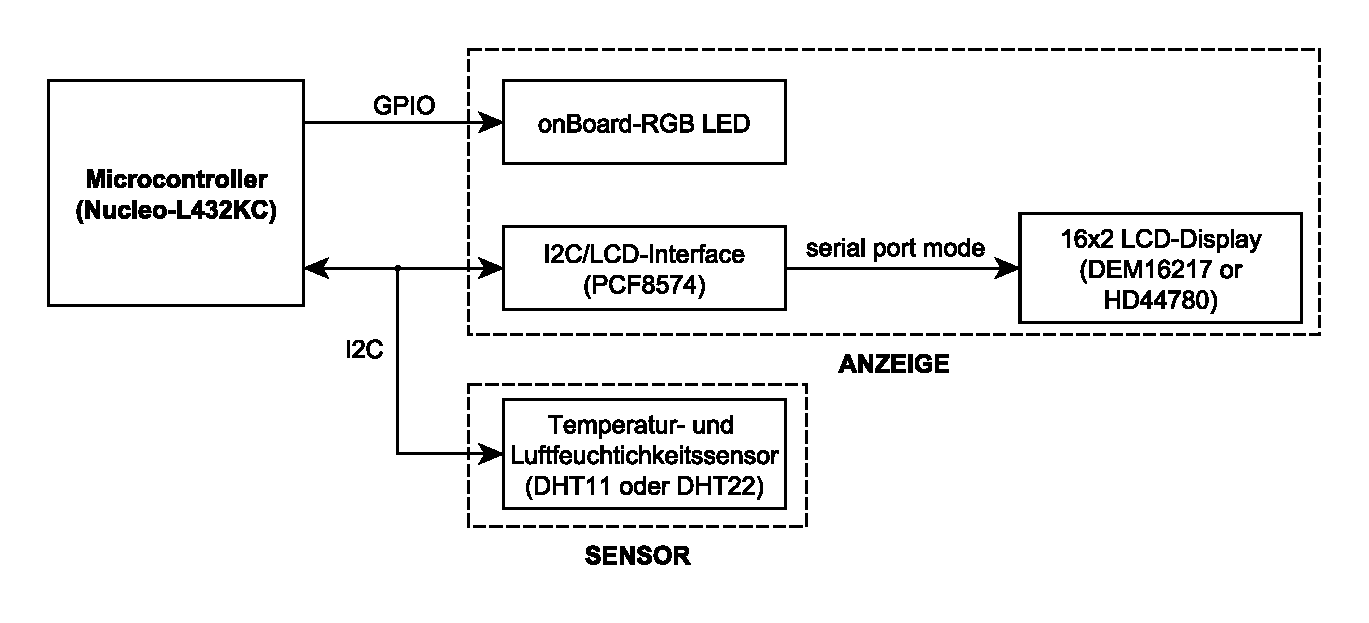
\includegraphics[width=0.8\linewidth]{Project_Mockup}
	\caption{Project Mockup}
	\label{figure:2}
\end{figure}

\pagebreak

\section{Spezielle Symbole}
Simple Low-High-Low \texttiming{[-,timing/slope=0]LHL} or Triangle \texttiming{[-,timing/slope=1]LHLL} with tikz \\
Or with ifsym \FallingEdge \\
also Temp.Symbole with gensymb \celsius \space \ohm \\
Hantelsymbol \laplace

\section{Diskussion}
Hier schreiben Sie, ob die Ergebnisse, die Sie bekommen haben, zu erwarten waren, vergleichen Sie die Berechnungen mit der 
Simulationen und Messungen, wenn sie nicht übereinstimmen, warum, usw. Diese muss nicht unbedingt eine eigene Abschnitt sein, 
das kann auch in Abschnitt \ref{sec:Experiment} hineinfließen.

\section{Cites and Acros}
Acros: \ac{FPGA}, \ac{ADC}, \ac{z.B.}\\
Glossars: \gls{gl:LTSpice}, \gls{gl:MATLAB}\\
Cites: \cite[85]{elekakustik}, \cite{rigoldg1000z}

\section*{Plagiat} % no Number
Plagiat ist die Arbeit von anderen als eigene Arbeit einzureichen, und ist streng verboten. Wenn ein Protokoll oder ein Teil davon 
identisch oder offensichtlich sehr ähnlich zu dem Protokoll anderer Gruppe ist, gilt als Plagiat. In dem Fall bekommen beide Parteien 
keine Punkte dafür, und es gibt keine Möglichkeit, dieses Protokoll wieder einzureichen oder zu verbessern.

\section{Zusammenfassung}
Wenn eine Person nur die Einleitung und die Zusammenfassung liest, soll sie einen groben Einblick bekommen, was Sie gemacht haben, 
welche Ergebnisse Sie bekommen haben, und ob sie zu erwarten waren oder nicht, und warum.

\newpage

\printbibliography
\listoffigures
\listoftables
\lstlistoflistings

\phantomsection
\addcontentsline{toc}{section}{\listacroname}
\section*{\listacroname}
\begin{acronym}[XXXXX]
    \acro{ADC}[ADC]{Analog Digital Converter}
    \acro{ASIC}[ASIC]{Application-Specific Integrated Circuit}
    \acro{BJT}[BJT]{Bipolar Junction Transistor}
    \acro{bzw.}[bzw.]{beziehungsweise}
    \acro{DAC}[DAC]{Digital Analog Converter}
    \acro{DUT}[DUT]{Device Under Test}
    \acro{FF}[FF]{Flipflop}
    \acro{FPGA}[FPGA]{Field Programmable Gate Array}
    \acro{LFSR}[LFSR]{Linear Feedback Shift Register}
    \acro{LUT}[LUT]{Look Up Table}
    \acro{MMI}[MMI]{Man Machine Interface}
    \acro{MSB}[MSB]{Most Significant Bit}
    \acro{MUX}[MUX]{Multiplexer}
    \acro{OPV}[OPV]{Operationsverstärker}
    \acro{PN}[PN]{Pseudo Noise}
    \acro{IP}[IP]{Intellectual Property}
    \acro{RAM}[RAM]{Random Access Memory}
    \acro{E/A}[E/A]{Eingabe/Ausgabe}
    \acro{I/O}[I/O]{Input/Output}
    \acro{IC}[IC]{Integrated Circuit}
    \acro{USB}[USB]{Universal Seriel Bus}
    \acro{uC}[\textmu C]{Mikrocontroller}
    \acro{uP}[\textmu P]{Mikroprozessor}
    \acro{VGA}[VGA]{Video Graphics Array}
    \acro{VHDL}[VHDL]{Very High Speed Integrated Circuit Hardware Description Language}
    \acro{XOR}[XOR]{eXclusiv-OR}
    \acro{z.B.}[z.B.]{zum Beispiel}
\end{acronym}

\newpage

\appendix % start Anhangkapitel
\section{Verwendete Programme}

\newglossaryentry{gl:LTSpice}
{
    name=LTSpice,
    description={Simulationsprogramm für analoge Schaltungen}
}

\newglossaryentry{gl:MATLAB}
{
    name=MATLAB,
    description={Programm zur automatisierten Erstellung der Cosinus -- \ac{LUT} und grafischen Darstellung}
}

\glsaddall
\setlength{\LTleft}{-5pt}
\renewcommand{\glsnamefont}[1]{\textbf{#1}}
\printglossary[title=Verwendete Programme, toctitle=Verwendete Programme,style=long,nonumberlist]

\section{Code}

\lstinputlisting[caption={Example Code Listing}, label = {lst:1}]{main.c}

\end{document}